\documentclass{article}

\usepackage{physics} % Handy shortcuts like \pdv, \dd and much more
\usepackage{geometry} % smaller margins, can be adjusted if given arguments
\usepackage{siunitx} % the \si environment for units
\usepackage{mathtools} % The dcases environment, prettier than just cases
\usepackage{tikz} % For drawing picures
\usepackage{wrapfig} % Wrapping text around figures


\title{Exercise x - TFY4345 Classical Mechanics}
\date{2020}

\begin{document}
    \maketitle
    \section{Binding energy of the deuteron}
    [This is a short one] \\
    Deuteron can be split by gamma rays in a nuclear experiment in the reaction $\gamma + {^2\mathrm{H}} \rightarrow p + n$. Calculate the energy required for the gamma rays for this process to occur, in electron volts. The quantities needed are
    \begin{itemize}
        \item Mass of a proton ($^1\mathrm{H} = p$): $1.007825 \si{u}$
        \item Mass of a neutron ($n$): $1.008665 \si{u}$
        \item Mass of deuteron ($^2 \mathrm{H}$): $2.014102$
        \item 1 \si{u} = 931.5 \si{MeV c^{-2}}
    \end{itemize}

    \section{Frequency shift on a rotating disk}
    \begin{wrapfigure}{2}{0.2\textwidth}
        \vspace{-1cm}
        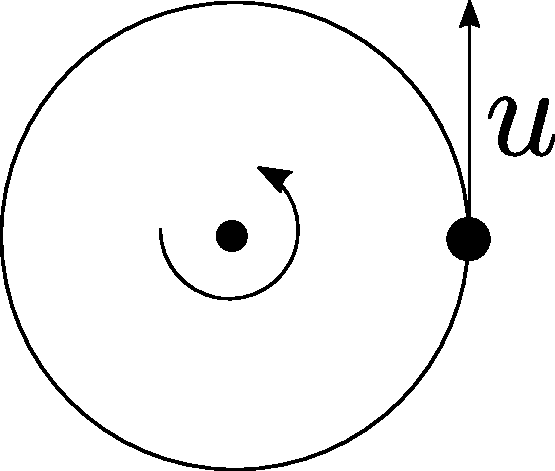
\includegraphics[width=0.2\textwidth]{figures/figure_1.pdf}
        \vspace{-1cm}
    \end{wrapfigure}
    A radioactive $^{57}\mathrm{Co}$ element is situated on the periphery of a rotating disk. The peripheral velocity is $u$. The radiation from the cobalt is received by an observer located in the center of the disk. Let $f_0$ be the eigenfrequency of the radiation in the the inertial system where the element is momentarily at rest. Find the frequency $f$ of the radiation observed by the observer in the center.
    
    \section{Fast moving particle in two inertial frames}
    [Exam Dec. 2019] \\
    We shall consider a particle with rest mass $m$ seen from two different inertial reference systems. In the reference system $s$, the particle has velocity
    \begin{equation*}
        \mathbf{u} = (u_x, u_y, u_z).
    \end{equation*} 
    The reference system $S'$ is moving along the $z$ axis with a velocity $v$ relative to the system $S$. In this frame, the particle has the velocity
    \begin{equation*}
        \mathbf{u'} = (u'_z, u'_y, u'_z).
    \end{equation*}
    Find the explicit relationship between $\mathbf{u}$ and $\mathbf{u'}$, i.e. derive the transformation that give $\mathbf{u'}$ from the components of $\mathbf{u}$. [Hint] Start with the relationship between the two frames, the Lorentz transformation. What is the definition of the components $u_i, \, u_j'$?

    \section{Lorentz transformation of energy and momentum}
    We shall consider a particle with res mass $m$ seen from two inertial reference systems, as in the last exercise. The systems $S$ and $S'$ has a relative velocity $v$ along the $z$-axis, and the particle has the constant velocity $\mathbf{u} = (u_x, u_y, u_z)$ and $\mathbf{u'} = (u_x', u_y', u_z')$ in $S$ and $S'$ respectively. \\ \\
    a) Einstein's velocity addition formulas are
    \begin{align*}
        u_x' = \frac{u_x}{\gamma(1 - v u_z/c^2)} \\
        u_y' = \frac{u_y}{\gamma(1 - v u_y/c^2)} \\
        u_z' = \frac{u_z - v}{1 - v u_z/c^2}
    \end{align*}
    (The difference between these, and the ones derived in the last exercise, is that they do not assume the third reference system e.g. the particle moves along the $z$-axis). Use these to show that
    \begin{equation*}
        \frac{1}{\sqrt{1 - u'^2/c}} = \gamma \frac{1 - v u_z / c^2}{\sqrt{1 - u^2/c^2}}.
    \end{equation*}
    Here, $\gamma = 1 / \sqrt{1 - v/c^2}$, $u^2= |\mathbf{u}| = u_x^2 + u_y^2 + u_z^2$ and $u'^2= |\mathbf{u}'|= u_x'^2 + u_y'^2 + u_z'^2$. \\ \\
    b) The energy E and 3-momentum $\mathbf{p}$ of the particle in the reference system $S$ is
    \begin{equation*}
        E = \frac{mc^2}{\sqrt{1 - (u/c)^2}}, \quad \mathbf{p} =\frac{m\mathbf{u}}{\sqrt{1 - (u/c)^2}},
    \end{equation*}
    while in the $S'$ system it is
    \begin{equation*}
        E' = \frac{mc^2}{\sqrt{1 - u'/c^2}}, \quad \mathbf{p'} =\frac{m\mathbf{u'}}{\sqrt{1 - u'/c^2}}.
    \end{equation*}
    Use the equation derived in a) to to find the transformation rule of energy of momentum, i.e. express $E'$ and $\mathbf{p}'$ in terms of $E$ and $\mathbf{p}$.
\end{document}
